The same system used in the experiment was used in the case study presented in this paper and they are explained in the following subsection. 

\subsection{Robotic Platform}

The non-anthropomorphic robotic platform was created to do not have any bio-inspired appearance. The holonomic platform was built using Odroid U3, Arduino Due, and 3 metal gear motors with 64 CPR encoders and omniwheels. The platform could be observed in Figure~\ref{fig:Robot}. The Arduino Due is in charge to be the interface between the hardware (e.g. motors) and Odroid, which host all the emotion enrichment system.

\begin{figure}[t]
\centering%
\subfigure {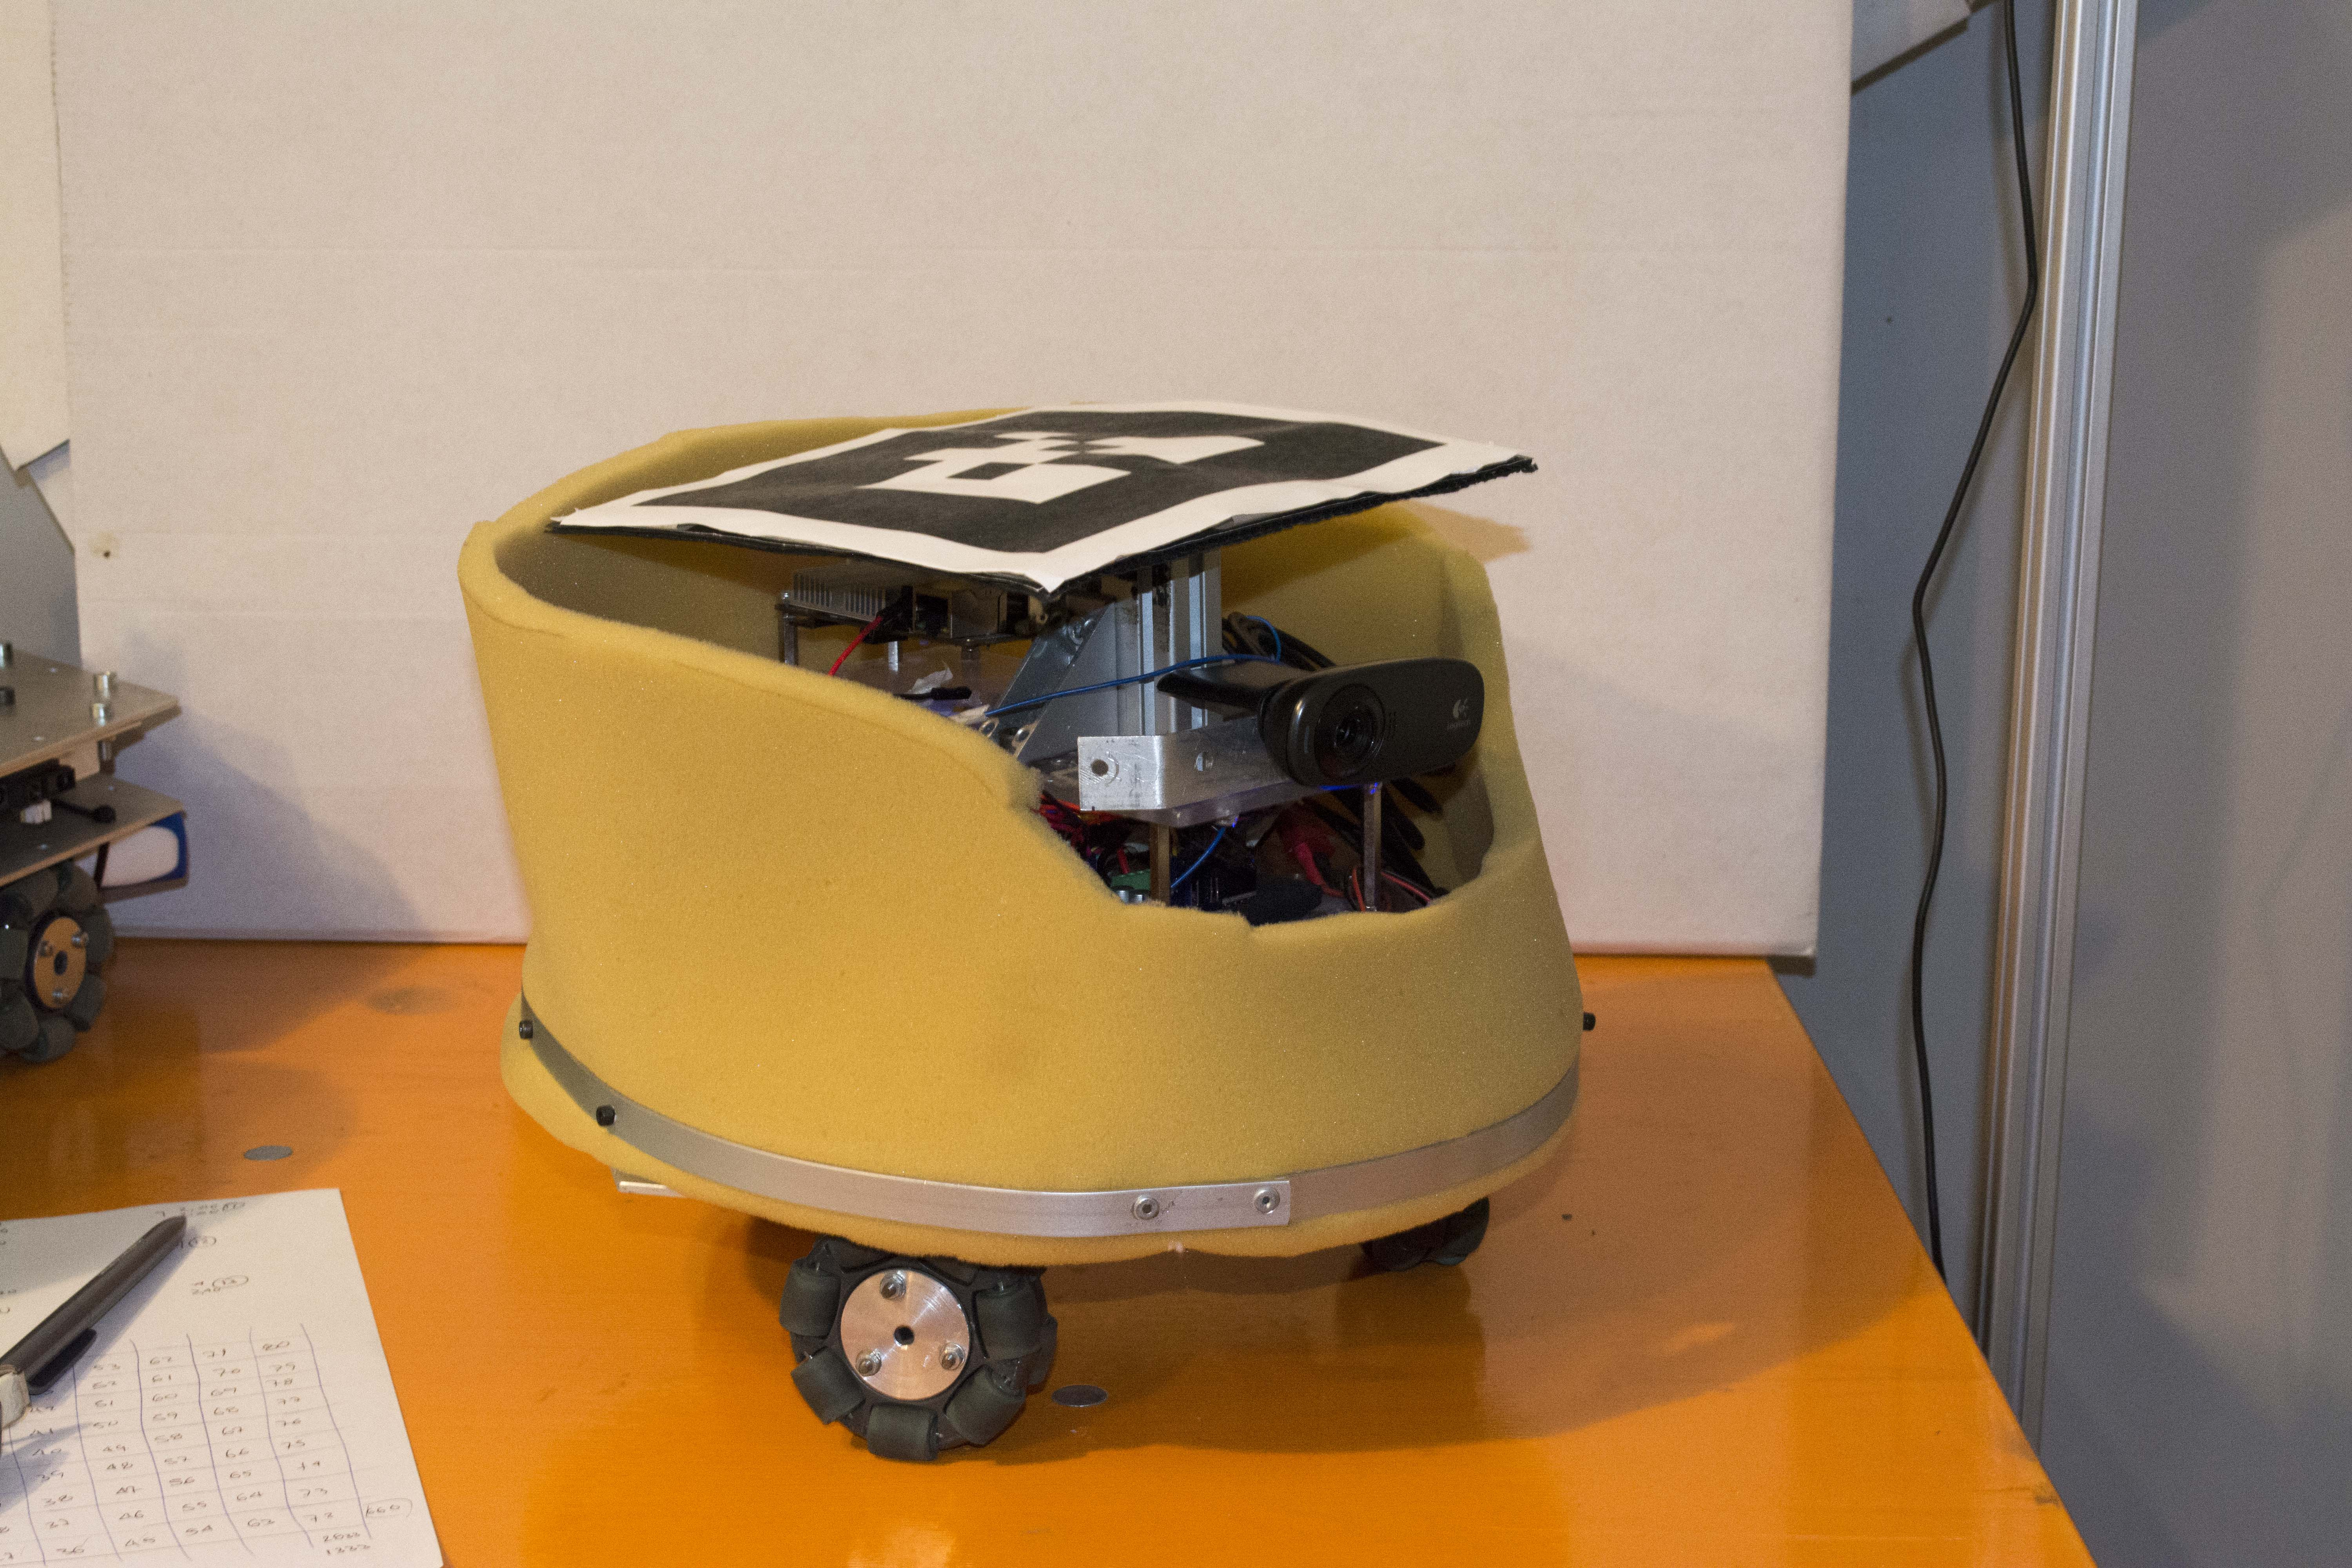
\includegraphics[height=3cm]{./Images/DSC_0447.JPG}}
\hspace{2mm}
\subfigure{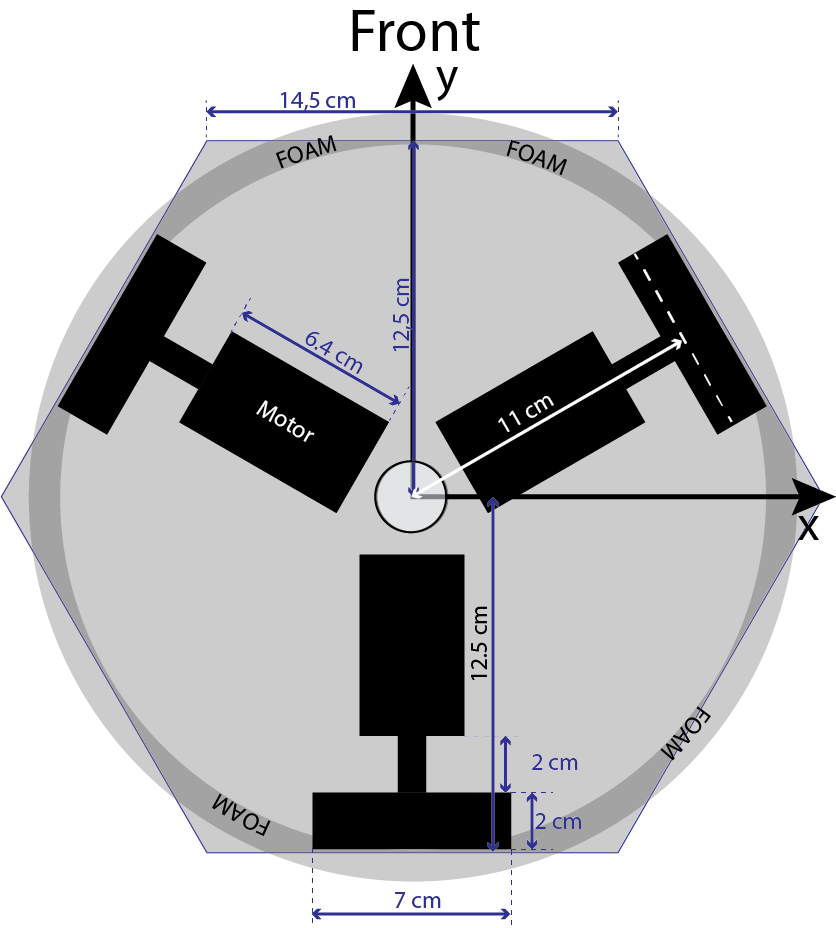
\includegraphics[height=3cm]{./Images/TriskarThird.png}}
\caption{Platform used in the case study (left), and holonomics's blue prints (right). The arrows represent robot's frame of reference.
\label{fig:Robot}}
\end{figure}

\subsection{Emotion Enrichment System}

The main idea of Emotional Enrichment System (EES) is to blend an emotion and a action to produce an "emotional action". However this is not far as previous works have done so far. Therefore, the system has been envisioned to also allow:

\begin{itemize}
	\item Interoperability among different platform.
	\item Introduction of new parameters and emotions.
	\item Interface with diverse action decision system.
\end{itemize}

In other words, the system could be thought as a box that receives a desire action, action's parameters and emotion to blend them together without paying particular attention on who or how the decision to execute a the particular action was made. This is achieved through the use of messages to describe the action that should be executed, as well its parameters, emotion and emotion's intensity.  These information are divided into two messages: one for the action and its parameters, and other for the emotion and its intensity. This is done to do not affect the action's execution.

Every time the system receives a new action, it verifies if the action exists and the parameters corresponds to the action. If these two conditions are met, then the system checks if the action is compound or simple. If it is a simple, the system proceeds to add all the required actions (emotive actions) and change their parameters to convey the desired emotion. On the other hand if the action is compound, the action is first decomposed in simple actions (mandatory actions). Each one of these actions is then process to add their emotive actions. However, this addition is done taking in consideration to not add any action that was previously added. Once all the set of simple actions and their parameters are determined, the system proceeds to verify the drivers' existence to execute these actions in the desired platform. If the system finds out that one or more mandatory actions could not be executed, it triggers a message to inform that the desire action could not be executed. 

%%%%%%%%%%%%%%%%%%%%%%%%%%%%%%%%%%%
\subsubsection{Simple and Compound Actions}

To achieve actions' enrichment with emotions, two different types of actions are used: simple and compound actions. Simple actions are actions that could be considered as ''atomic''; these actions can be enriched with emotion changing their specific parameters. For example, consider two simple actions: speak and move body. The human action of speaking is related to changes in the vocal cords to produce different sounds, while move body is directly related to the body movement. Therefore, for the speaking action the following parameters are expected: text, pitch and tone. On the other hand, the action move body would have as parameters the desired destination, velocity, and trajectory constraints. Since each action is characterized by different parameters, the parameters' modifications to obtain an emotional action will be different for each of them. On the other hand, compound action is an action created from other compound or simple actions. For example, suppose that it is required that the robot has to \textit{recite} some dialogue and \textit{walk} to a different position, as doing a trajectory. A possible implementation could consist on speak simple action in parallel to two consecutive action walk, which is also a compound action that is composed by three parallel actions: balance left arm, balance right arm, and move body.

Although compound actions could be used to generate diversity of actions from simple actions, the main drawback of this approach is that all possible combination of actions should code in the system to be used. Using the example previously described, if it is decided to have three positions instead of two, then it would mean that a new compound action should be implemented to have an action in which could be specified three positions. To overcome this limitation, it was created a language to specify actions that are not implemented in the system. A computational representation of these language is used to execute the actions described in this language. 

\subsubsection{Emotional Execution Tree}
The \textit{Emotional Enrichment System}  is grounded on the use of \textit{Emotional Execution Tree} ($EXT$), which is a computational representation of desired actions that must be executed. 
$EXT$ is a connected acyclic graph with vertices and  edges. The root and non-leaf nodes could be \textit{parallel} or \textit{sequence} type. The parallel node could be one out of four different sub-types: action and emotion synchronous, action synchronous and emotion asynchronous, action asynchronous and emotion synchronous, or action and emotion asynchronous. Sequential nodes could just be one of two sub-types: emotion synchronous or asynchronous. Action synchronous means that each time that a parallel node receives a finish notification (success or failure), it will send a finish message to all the nodes that derived from it. On the other hand, emotion synchronous means that each time that a node (sequence or parallel) receives an emotion synchronization message, it will propagate the message to all the actions in the branches. 
This distinction creates the possibility to synchronize emotional changes without affecting the normal execution of the desired action. Finally, the leaf nodes could only be simple action nodes. All the nodes can assume two levels: principal or secondary. If a node is principal, it will notify its predecessor about the messages that it has received, while the secondary cannot propagate any message to its predecessor.

\subsubsection{Implementation}
Figure~\ref{fig:system_architecture} presents the design used to achieve the desire goals. As it could be observed, the system is divided in two parts. The first part in charge to enrich a given action with a desired emotion, and the second in charge to hide the real execution of the action. 

\begin{figure*}
	\centering
	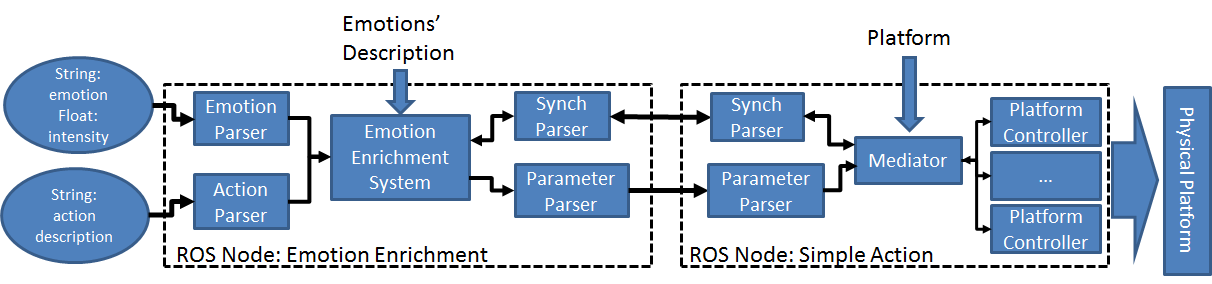
\includegraphics[width=1.0\textwidth]{Images/SystemArchitecture.png} 	
	\caption{General system design. Each simple action corresponds to one ROS node, and there is just one node for the emotion enrichment system. The ovals represent the ROS topic parameters, rectangles represent \textit{black boxes}, and texts outside containers represent input files that contain the system parametrization.}
	\label{fig:system_architecture}
\end{figure*}

The action enrichment is achieved through the following phases:
\begin{enumerate}

	\item \textit{Generation of emotional execution tree:} this phase starts every time that a new action message is received. The process begins by parsing the format, verifying that the actions described on it exist in the system, and that the parameters correspond to the ones expected by each action described in the message. This parameters' verification is done on the implemented description for each simple action, which describes the parameters that are mandatory and those that are optional. When the verification is done, and all the action exists and  the parameters correspond, an $ext$ is created.

	\item \textit{Emotion addition:} uses the $ext$ created in the previous phase. In this phase new simple actions are added to the $ext$ and the simple action's parameters are modified following the emotion description, which is loaded from files. This process is broken down in two steps. First, all actions that are required to convey the desired emotion, and that are not yet present in the branch are added. Second, the emotional parameters are modulated based on the emotion's intensity and character traits.

	\item \textit{Execution:} this is the last phase and it is done after the $ext$ is ''coloured'' with emotional characteristics (actions additions and emotional parameters). The decision to have two different communication channels, one for action parameters and another for the action emotional parameters, was taken to enable the possibility to update the emotional parameters without interfering with the current execution. In this phase is maintain a reference to the mandatory and emotional action, thus when a new emotion is received the system stops the previous emotional action and start executing the new ones without affecting the general execution of the actions.

\end{enumerate}